% -------------------------------------------------------------------------
\begin{frame}{Introduction}
\begin{center}
\block{What is HPC?}
\begin{itemize}
  \item Powerful processors in parallel
  \item Handle large-scale data and solve complex problems
  \item High computational throughput
\end{itemize}
\endblock{}
\begin{figure}[H]
	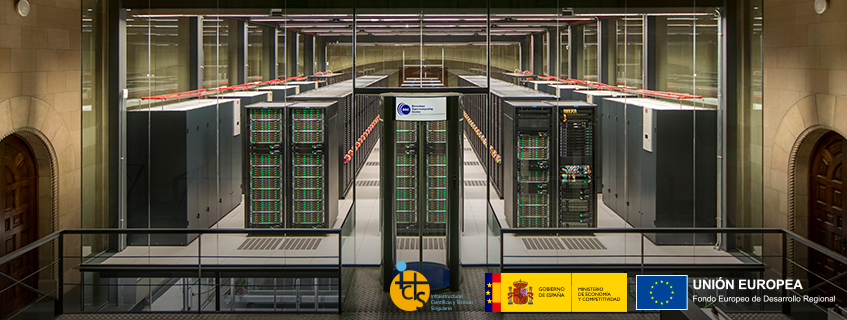
\includegraphics[width=0.65\linewidth]{Images/mare-nostrum.png}
\end{figure}
MareNostrum supercomputer in Barcelona. \textit{(Credit: \url{www.bsc.es})}
\end{center}
\end{frame}
% -------------------------------------------------------------------------
\begin{frame}{Introduction}
\begin{center}
\block{Motivation \& Objectives}
\begin{itemize}
  \item Gain knowledge in HPC
  \item Learn about the parallel programming model
  \item Study and apply the SYCL language
\end{itemize}
\endblock{}
\end{center}
\end{frame}
% -------------------------------------------------------------------------
\begin{frame}{Introduction}
  Nowadays, there is a wide variety of devices specialized in different types of computing tasks (CPU, FPGA, GPU, ASIC, etc.)
\begin{block}{}
With the vast amount of devices comes the also varied collection of
APIs
\end{block}
\begin{center}
	
\includegraphics[width=0.3\linewidth]{Images/opencl-logo.png}
	
\includegraphics[width=0.4\linewidth]{Images/cuda-logo.png}
	
\includegraphics[width=0.4\linewidth]{Images/openacc-logo.png}
	
\includegraphics[width=0.4\linewidth]{Images/openmp-logo.png}
\end{center}
\end{frame}  
% -------------------------------------------------------------------------